\documentclass[11pt,a4paper]{article}

% \usepackage{polski}
\usepackage[utf8]{inputenc}

\usepackage[left=2cm, right=2cm, top=1cm, bottom=2cm]{geometry}

\usepackage{graphicx}
\usepackage{mathtools}
\usepackage{amssymb}
\usepackage{amsthm}
\usepackage{thmtools}
\usepackage{xcolor}
\usepackage{nameref}
\usepackage{babel}
\usepackage{hyperref}
\usepackage{enumitem}
\usepackage{amsmath, amsthm}
\usepackage{booktabs}
\usepackage{float}

\usepackage{listings}
\lstset{
  language=R,
  basicstyle=\ttfamily\small,
  keywordstyle=\color{blue},
  commentstyle=\color{gray},
  stringstyle=\color{orange},
  numbers=left,
  numberstyle=\tiny,
  breaklines=true,
  captionpos=b
}

% Definicje nowych środowisk
\newtheorem{theorem}{Theorem}
% \newtheorem{lemma}{Lemat}
% \newtheorem{fact}{Fakt}
% \newtheorem{corollary}{Wniosek}
% \newtheorem{exercise}{Zadanie}[subsection]
% \newtheorem{solution}{Rozwiązanie}
% \newtheorem{definition}{Definicja}
% \newtheorem{namedtheorem}{Twierdzenie}[subsection]
% \newtheorem{example}{Przykład}

\newcommand{\PP}{\mathbb P}
\newcommand{\EE}{\mathbb E}
\newcommand{\Z}{\mathbb Z}
\newcommand{\R}{\mathbb R}
\newcommand{\Poi}{\mathrm{Poiss}}
\newcommand{\F}{\mathcal F}
\newcommand{\tn}{{\tau \wedge n}}
\newcommand{\var}{\mathrm{Var}}
\newcommand{\cov}{\mathrm{Cov}}
\newcommand{\N}{\mathbb N}

\begin{document}

    \title{Time Series Final Assessment \\ Exercise 6: Forecasting of the USD/EUR Exchange Rate}
    \author{Kacper Omieliańczyk}
    \date{}

    \maketitle
    
    \section{Exploratory Data Analysis}
    \label{chap:eda}

    In this section we explore the USD/EUR exchange-rate data over 2008-2014 to understand its main features, guide our modeling choices, and lay the groundwork for one-step-ahead forecasting. We work in both price (level) space and log-return space.

    \subsection{Data Description}
    The data consist of 264 weekly observations of the USD/EUR exchange rate from early 2008 through mid-2014.  We denote by \(p_t\) the rate on date \(t\).  After parsing and cleaning, our working data frame has two columns:
    \begin{itemize}
    \item \texttt{Date}: the week's ending date.
    \item \texttt{Price}: the USD/EUR rate \(p_t\).
    \end{itemize}

    \subsection{Descriptive Statistics of Prices}
    Table~\ref{tab:annual_stats} shows, for each calendar year, the sample size, mean, standard deviation, minimum, maximum, skewness and excess kurtosis of the weekly closing rate.
    \begin{table}[H]
    \centering
    \caption{Annual summary statistics of USD/EUR (Price)}  
    \label{tab:annual_stats}
    \small
    \begin{tabular}{rrrrrrrr}
        \toprule
        Year & \(n\) & Mean & SD & Min & Max & Skewness & Kurtosis \\ 
        \midrule
        2009 &   32 & 0.694 & 0.0183 & 0.666 & 0.729 & 0.007  & -1.37 \\ 
        2010 &   52 & 0.754 & 0.0351 & 0.691 & 0.832 & 0.302  & -0.79 \\ 
        2011 &   52 & 0.718 & 0.0234 & 0.680 & 0.766 & 0.331  & -1.06 \\ 
        2012 &   53 & 0.778 & 0.0196 & 0.748 & 0.821 & 0.558  & -0.86 \\ 
        2013 &   52 & 0.753 & 0.0145 & 0.727 & 0.777 & -0.116 & -1.14 \\ 
        2014 &   19 & 0.728 & 0.0056 & 0.720 & 0.738 & 0.346  & -1.33 \\ 
        \bottomrule
    \end{tabular}
    \end{table}

    \paragraph{Insights.}
    \begin{itemize}
    \item The rate dipped during the 2008-2009 crisis (2009 mean 0.694) then climbed through 2012 (mean 0.778).
    \item Volatility (SD) peaked in 2010 (0.035) and declined thereafter.
    \item All years exhibit slight negative excess kurtosis (platykurtic) and mild skew.
    \end{itemize}

    \subsection{Time-Series Plots}
    Figure~\ref{fig:ts} shows the weekly closing rate over the full sample.

    \begin{figure}[H]
    \centering
    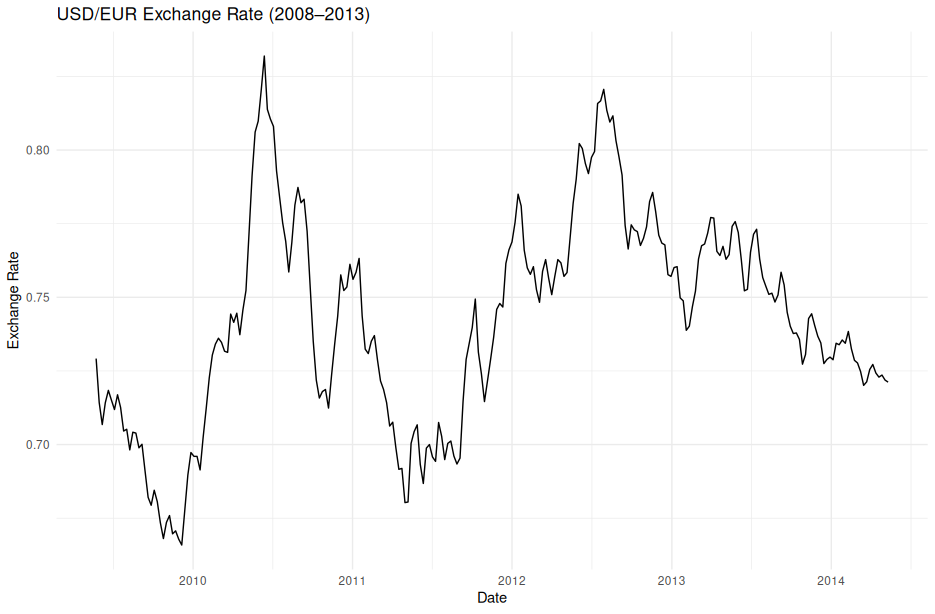
\includegraphics[width=0.8\textwidth]{figures/usdeur_timeseries.png}
    \caption{USD/EUR exchange rate, weekly closes (2008-2014).}
    \label{fig:ts}
    \end{figure}

    Notable features:
    \begin{itemize}
    \item A trough near mid-2009 (\(\approx0.667\)), and a peak in late 2010 (\(\approx0.83\)).
    \item A secondary peak around mid-2012 (\(\approx0.82\)).
    \item A gradual decline after 2012 toward \(\approx0.72\) by mid-2014.
    \end{itemize}

    Figure~\ref{fig:ma} overlays a 30-week moving average to highlight medium-term trends.

    \begin{figure}[H]
    \centering
    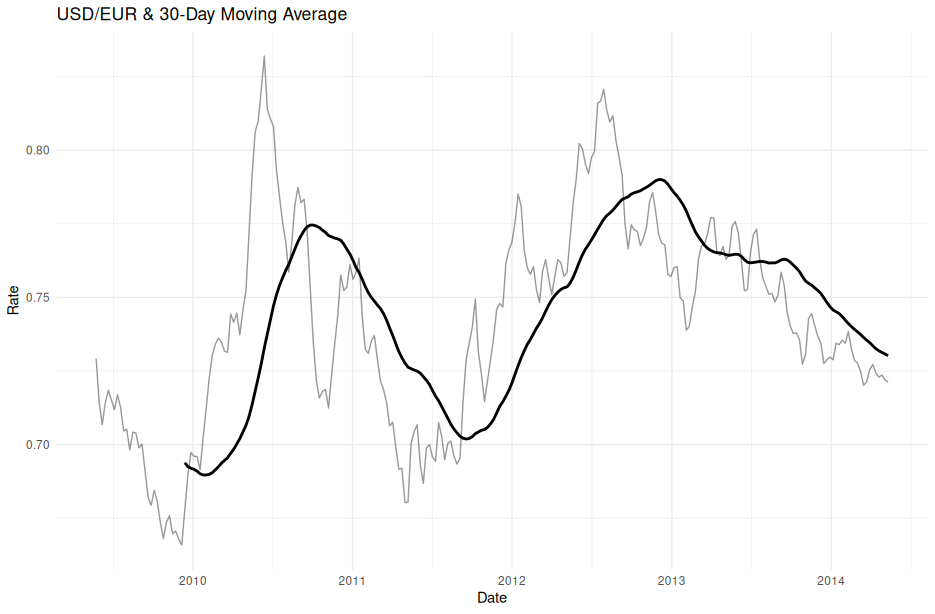
\includegraphics[width=0.8\textwidth]{figures/usdeur_ma30.png}
    \caption{USD/EUR and its 30-week moving average.}
    \label{fig:ma}
    \end{figure}

    \subsection{Distribution by Year}
    To compare variability and location year-by-year, Figure~\ref{fig:box} presents boxplots of the weekly rate by calendar year.

    \begin{figure}[H]
    \centering
    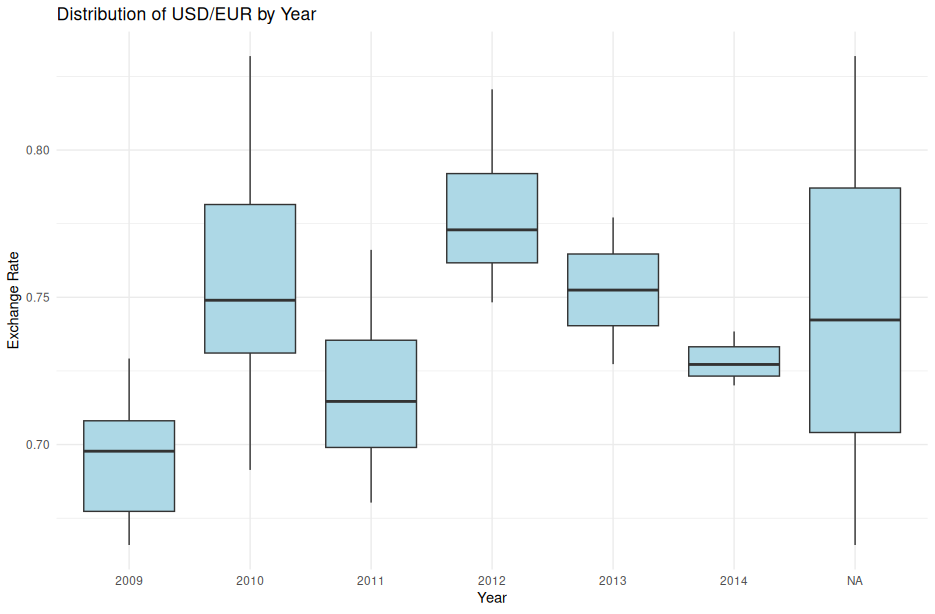
\includegraphics[width=0.8\textwidth]{figures/usdeur_boxplot_year.png}
    \caption{Distribution of USD/EUR by year (2009-2014).}
    \label{fig:box}
    \end{figure}

    \subsection{Log-Return Analysis}
    We define the log-return \(r_t = \ln(p_t) - \ln(p_{t-1})\).  Table~\ref{tab:return_stats} reports annual summaries.

    \begin{table}[H]
    \centering
    \caption{Annual summary statistics of USD/EUR log-returns}
    \label{tab:return_stats}
    \small
    \begin{tabular}{rrrrr}
        \toprule
        Year & Mean & SD & Min & Max \\ 
        \midrule
        2009 & -0.00144 & 0.00939 & -0.0206 &  0.0177 \\ 
        2010 &  0.00169 & 0.0128  & -0.0249 &  0.0255 \\ 
        2011 &  0.00012 & 0.0121  & -0.0259 &  0.0288 \\ 
        2012 & -0.00022 & 0.00912 & -0.0218 &  0.0202 \\ 
        2013 & -0.00071 & 0.00791 & -0.0147 &  0.0166 \\ 
        2014 & -0.00062 & 0.00416 & -0.0080 &  0.0077 \\ 
        \bottomrule
    \end{tabular}
    \end{table}

    Figure~\ref{fig:returns} shows the return series and its distribution.

    \begin{figure}[H]
    \centering
    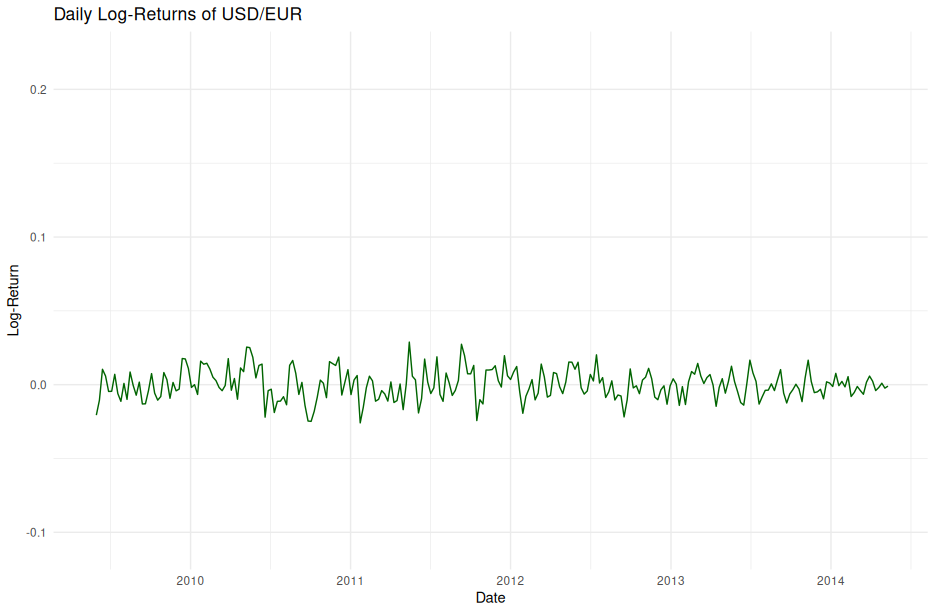
\includegraphics[width=0.8\textwidth]{figures/usdeur_returns_timeseries.png}
    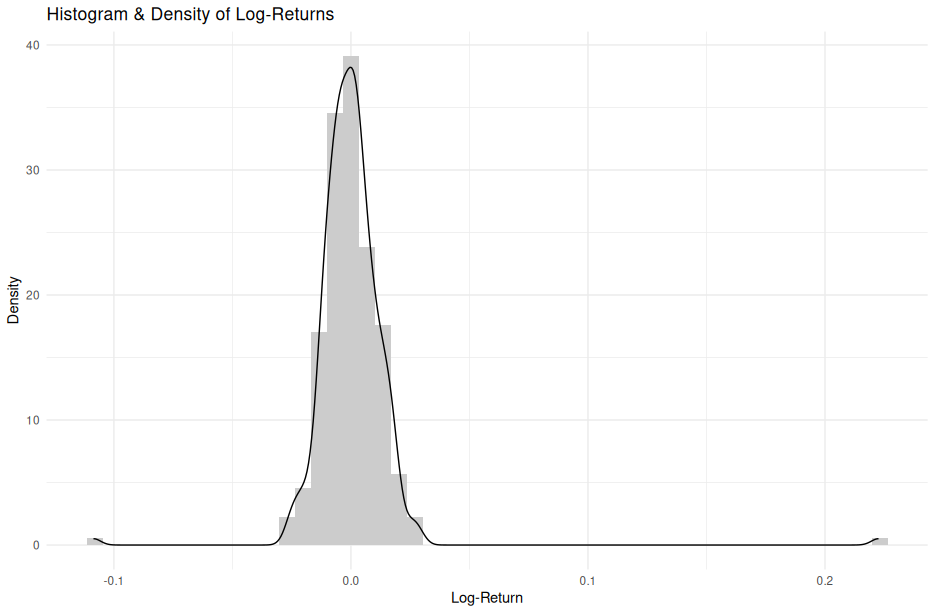
\includegraphics[width=0.8\textwidth]{figures/usdeur_returns_hist.png}
    \caption{Top: log-returns over time.  Bottom: histogram \& kernel density.}
    \label{fig:returns}
    \end{figure}

    \paragraph{Insights.}
    \begin{itemize}
    \item Returns are tightly centered around zero, with SD decreasing from 2010 onward.
    \item Distribution is mildly leptokurtic with occasional large moves (|\(r_t\)| up to 2–3\%).
    \end{itemize}

    \subsection{Stationarity and Autocorrelation}
    Augmented Dickey-Fuller tests indicate
    \[
    \text{ADF}(\{p_t\})\;p\text{-value}=0.338
    \quad\text{(non-stationary)}, 
    \quad
    \text{ADF}(\{r_t\})\;p\text{-value}=0.01
    \quad\text{(stationary).}
    \]
    Thus we will model in log-return space.

    Figure~\ref{fig:acf_pacf} displays ACF and PACF of \(\{r_t\}\) up to lag 25.

    \begin{figure}[H]
    \centering
    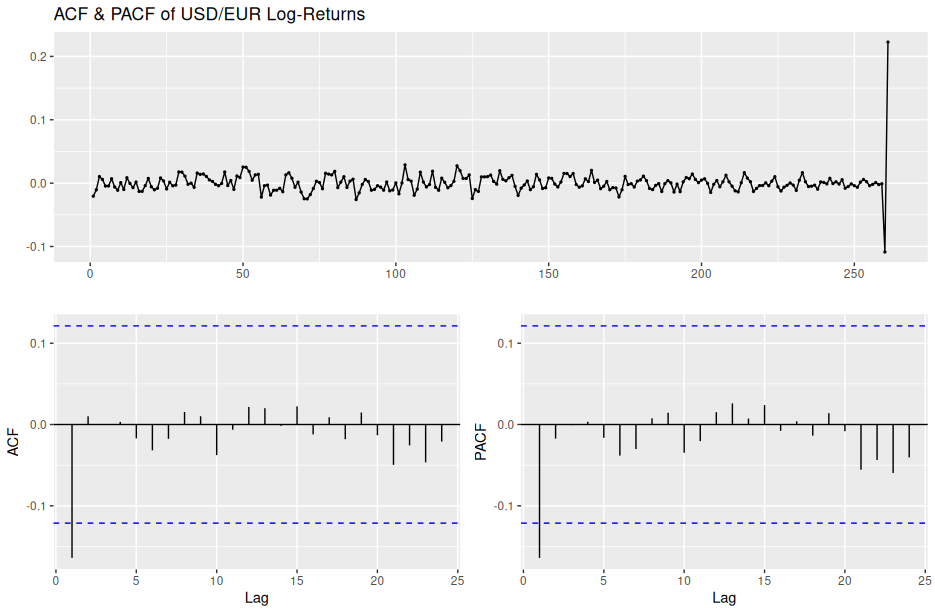
\includegraphics[width=0.8\textwidth]{figures/usdeur_acf_pacf.png}
    \caption{ACF (left) and PACF (right) of USD/EUR log-returns.}
    \label{fig:acf_pacf}
    \end{figure}

    The first-order autocorrelation is slightly negative (\(\approx -0.15\)), with most higher lags within the 95\% bounds.

    \subsection{Conclusions and Next Steps}
    Based on the EDA:
    \begin{itemize}
    \item The level series is non-stationary; log-returns are stationary.
    \item Returns exhibit low autocorrelation beyond lag 1, suggesting an AR(1) or simple EWMA could be competitive.
    \item Volatility clusters in 2009-2011 but calms thereafter; a simple GARCH(1,1) may yield marginal improvements.
    \item We will proceed to one-step-ahead forecasts in return space, benchmarked against naive, SES, ARIMA(1,0,1), and (optionally) GARCH‐type models, comparing by sum of squared errors.
    \end{itemize}

    This completes our exploratory analysis and paves the way for the full forecasting exercise.  

    \subsection{R code}
    This is the used EDA R code:
    \lstinputlisting[
    language=R,
    caption={EDA for USD/EUR},
    label={lst:eda_external},
    ]{exercise6_eda.R}

    \section{One-Step-Ahead Forecasting}
    \label{sec:forecasting}

    In this section we describe our recursive forecasting setup, the five candidate models we evaluated (Random-Walk, SES, Holt's linear, ARIMA, and GARCH(1,1)), and the out-of-sample results on a one-year holdout.  We work in log-return space, back-transform to prices, and compare by the sum of squared forecast errors (SSE).

    \subsection{Forecasting Framework}
    We choose two consecutive years, 2010 as the \emph{training} (burn-in) period and 2011 as the \emph{testing} (forecasting) period.  Let \(p_t\) be the observed USD/EUR rate on date \(t\), and
    \[
    r_t \;=\;\ln(p_t)\;-\;\ln(p_{t-1})
    \]
    the log-return.  For each week \(t\) in 2011 we:

    \begin{enumerate}
    \item Fit each candidate model on all returns \(\{r_1,\dots,r_{t-1}\}\) up to the previous date.
    \item Produce a one-step-ahead forecast for the return, \(\hat r_t\).
    \item Back-transform to a price forecast
        \[
        \hat p_t \;=\; p_{t-1}\,\exp\!\bigl(\hat r_t\bigr).
        \]
    \end{enumerate}

    We then compute the loss
    \[
    \mathrm{SSE} \;=\;\sum_{t\in\mathrm{test}} (p_t - \hat p_t)^2
    \]
    for each model over all 52 weeks in 2011.

    \subsection{Candidate Models}
    We considered five methods, all fitted to the log-return series:

    \begin{description}[itemsep=1ex]
    \item[Random-Walk (Naive)] \hfill\\
        \(\displaystyle\hat r_t = 0\).  The standard naive benchmark.
    \item[Simple Exponential Smoothing (SES)] \hfill\\
        An ETS(\(\text{A},\text{N},\text{N}\)) model on \(\{r_t\}\).
    \item[Holt's Linear Method] \hfill\\
        An ETS(\(\text{A},\text{A},\text{N}\)) model capturing trend in returns.
    \item[ARIMA] \hfill\\
        The \(\mathrm{ARIMA}(p,0,q)\) automatically selected by \texttt{auto.arima()}.
    \item[GARCH(1,1)] \hfill\\
        A GARCH(1,1) model on \(\{r_t\}\) with constant mean, capturing volatility clustering.
    \end{description}

    \subsection{Out-of-Sample Results}
    Table~\ref{tab:forecast_sse} reports the sum of squared errors for each model on the 2011 holdout:

    \begin{table}[H]
    \centering
    \caption{Sum of squared forecast errors (SSE) for 2011}
    \label{tab:forecast_sse}
    \small
    \begin{tabular}{l r}
        \toprule
        Model              & SSE         \\ 
        \midrule
        Random‐Walk (RW)   & 0.00388     \\ 
        SES                & 0.00451     \\ 
        Holt’s Linear      & 0.00436     \\ 
        ARIMA              & \(\mathbf{0.00379}\)  \\ 
        GARCH(1,1)         & 0.00388     \\ 
        \bottomrule
    \end{tabular}
    \end{table}

    The ARIMA model achieved the lowest SSE, with the GARCH(1,1) model matching the naive Random-Walk benchmark.

    Figure~\ref{fig:forecast_plot} overlays the actual USD/EUR rates in 2011 against the ARIMA forecasts:

    \begin{figure}[ht]
    \centering
    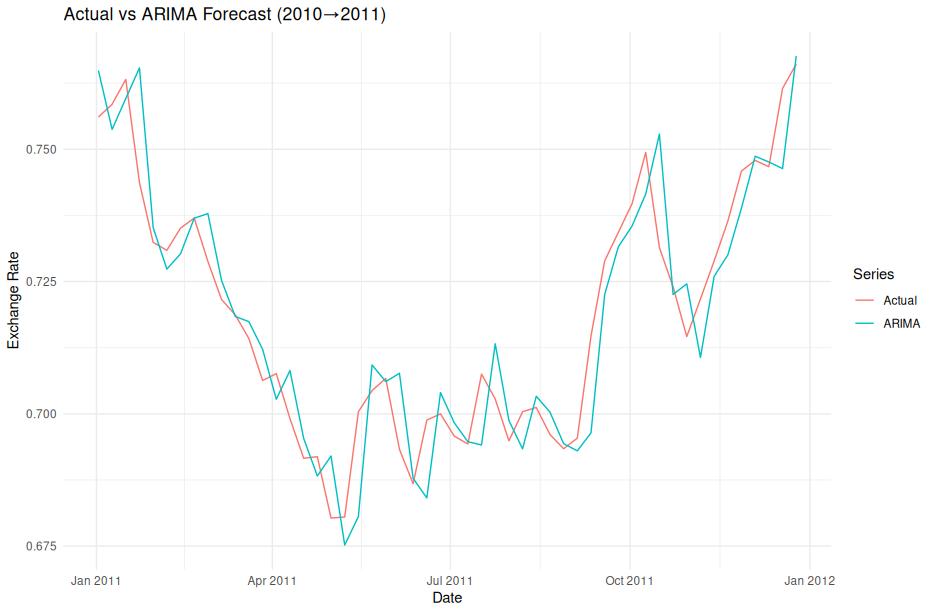
\includegraphics[width=0.85\textwidth]{figures/best_forecast_arima_2010_2011.png}
    \caption{Actual vs.\ ARIMA one-step-ahead forecasts (training on 2010, testing on 2011).}
    \label{fig:forecast_plot}
    \end{figure}

    \subsection{Discussion}
    \begin{enumerate}[label=(\alph*), itemsep=1ex]
    \item \emph{Price vs.\ return space:}  
        The level series \(p_t\) is non-stationary (ADF \(p\approx0.34\)), whereas the log-returns \(r_t\) are stationary (ADF \(p\approx0.01\)).  Modeling in return space stabilizes variance and satisfies stationarity requirements; forecasts are then back-transformed to price for evaluation.
    \item \emph{Parsimony vs.\ complexity:}  
        Among the five methods, the low-order ARIMA provided the best out-of-sample accuracy.  The GARCH(1,1) model—despite explicitly modeling volatility clustering—offered no improvement over the Random-Walk.  This highlights that added complexity (more parameters) does not guarantee better point forecasts.
    \item \emph{Statistical vs.\ economic significance:}  
        The ARIMA forecast reduced SSE by about 2.3\% relative to the Random-Walk.  In FX markets, even such a small predictive edge can be operationally valuable, though transaction costs and execution risk may erode gains.
    \item \emph{Robustness and future work:}  
        We might extend the framework by exploring time-varying parameter models, regime-switching, or machine learning methods with engineered features.  Incorporating macroeconomic predictors or news-based sentiment could further enhance forecast performance.
    \end{enumerate}

    \subsection{Conclusion}
    Across all five candidate models, a simple ARIMA on log-returns delivered the lowest SSE and thus the most accurate one-step-ahead forecasts for 2011.  Volatility modeling via GARCH(1,1) did not improve point-forecast performance, reinforcing that parsimony often prevails in exchange-rate prediction.  Future enhancements could focus on hybrid or regime-aware approaches to capture market dynamics beyond linear autocorrelation.  

    \subsection{R code}
    This is the used R code for forecasting:
    \lstinputlisting[
    language=R,
    caption={Forecast for USD/EUR exchange rate},
    label={lst:forecast_external},
    ]{exercise6_forecast.R}

\end{document}